\documentclass[output=paper]{LSP/langsci}  
\author{Tyler Kendall\affiliation{University of Oregon}\and Valerie Fridland\affiliation{University of Nevada, Reno}} 
\title{Mapping the perception of linguistic form: {D}ialectometry with perceptual data}
\abstract{In this paper we examine the geographic distribution of perceptual data from over 550 participants from around the U.S. in an experiment testing the categorical perception of vowel continua across several word pairs (e.g. \textit{bet}{\textasciitilde}\textit{bait}, \textit{bid}{\textasciitilde}\textit{bead}, \textit{sad}{\textasciitilde}\textit{sod}). Previous research has demonstrated that vowel identification, at least for certain vowel pairs like /e/ and /ɛ/, is significantly different across the major dialect regions of the U.S. and that vowel identification can be influenced by individual participants’ own vowel configurations in production \citep{fridland_exploring_2012}. Here, we focus for the first time on the actual geographic distribution of the participants, to ask to what extent modern methods of dialectometry, in particular spatial autocorrelation \citep{grieve_statistical_2011}, can help us to understand these data, and the regional patterning of perception differences more generally.

}
\rohead{Mapping the perception of linguistic form}
\maketitle 
\begin{document}

 

% \begin{multicols}{2}
% 
% Tyler Kendall\\
% 
% 
% Valerie Fridland\\
% 
% \end{multicols}
 
\section{Introduction}
In this paper we consider how methods from dialectometry\is{dialectometry|(} can aid our understanding of regional differences in perception by geospatially examining the results from a large-scale, web-based vowel identification experiment, where listeners throughout many parts of the U.S. were asked to identify which word they heard when stimuli were played with synthesized and somewhat ambiguous vowel acoustics (e.g. a range between \textit{bait}{\textasciitilde}\textit{bet}). This work comes from a larger, long-term project in which we have sought to understand regional differences in the perception of U.S. English vowels and linkages between perception and production at both the regional and individual level \citep{fridland_exploring_2012,kendall_mapping_2010,kendall_variation_2012}, as well as lesser studied aspects of the vowel systems of U.S. English (e.g. \citealt{fridland_durational_2014}). Those projects have identified a number of regional patterns in perception. For instance, in \cite{kendall_variation_2012} we identified that Southerners performed significantly differently from non-Southerners for the vowel continua probing the relationship between the mid-front vowels, /e/ and /ɛ/. In the present paper, we turn our attention to recent developments in dialectometry, the statistical evaluation and visualization of geographic variation in language, to ask whether we can shed better, more granular light on the regional distribution of perceptual patterns in our data. 

In terms of speech production in the traditional domain of dialectology, researchers have long utilized mapping techniques to isolate the use of a feature or form in geographic space. In doing so, dialectology has brought to light much about the way such features interact with social and geographic barriers and, in wave or gravity models, about the way change spreads across space and time (cf. \citealt{chambers_dialectology_1998}). Recent work in understanding regional variation has increasingly focused on quantitative and statistical approaches to the analysis and mapping of regional forms. This work, under the heading \textsc{dialectometry}, has developed more sophisticated approaches to understanding the regional distribution of variants (cf. \citealt{lee_spatial_1993}; \citealt{nerbonne_introducing_2003}; \citealt{nerbonne_data-driven_2009}; \citealt{szmrecsanyi_grammatical_2012}) and intersected modern dialectological work with advances in geographical information systems (GIS\is{geographic information system (GIS)}) more generally. It has also allowed researchers to take advantage of the vast accumulations of dialectological data now available. However, mapping perception is still in its infancy and researchers have not explored whether the same techniques that have been used on production data by linguistic geographers so successfully might be as useful for understanding regional variation in perception.   
In this paper, we attempt to tease out some of the ways in which the methods utilized in production contexts can be used to illuminate if and how perception maps across space. We largely draw on work from dialectometry, and in particular recent work by Jack Grieve and colleagues \citep{grieve_corpus-based_2009,grieve_statistical_2011,grieve_multivariate_2013}, which applies \textsc{\isi{geospatial autocorrelation}} \textsc{techniques} to assess regional patterns in (typically productive) language data. As we consider the future of dialects and dialectology, we hope the work here can suggest new uses for geospatial mapping techniques and also illustrate the value of looking past production to perception in assessing dialect differences. Can these approaches help us identify patterns in perception across and within more traditionally defined dialect regions (e.g. \citealt{carver_american_1987}; \citealt{labov_atlas_2006-1})? Can we find significant regional patterns in perception like we do for production?

\section{Background}
To begin to look at the question of whether we can identify regional differences in perception using approaches from dialectology in general and the quantitative methods of dialectometry\is{dialectometry|)} in particular, we first consider previous dialectological work that has focused on perception. Perhaps the best-known work of this kind is the approach, aptly named \textsc{\isi{perceptual dialectology}}, pioneered by Dennis Preston (\citeyear{preston_perceptual_1989,preston_folk_1993}). In this type of study, participants are given a map and asked to label where or how people speak differently. Perceptual dialectology is, at its heart, the study of folk-linguistic beliefs (cf. \citealt{niedzielski_folk_1999}), correlating overt attitudes and beliefs of speakers with specific locations or regions on a map. Generally, such work finds that listeners’ negative attitudes tend to have geographic correlates, namely in the areas where stereotyped dialects are believed to be regularly spoken. For example, in Preston’s work (e.g. \citeyear{preston_perceptual_1989}), negative attitudes toward Southern speech keenly affected how states in the South were rated in intelligence and education compared to non-Southern states. On the other hand, the same areas tended to suffer less on ratings of pleasantness. Thus, in such work we see that dialect regions, despite having a great deal of social and ethnic diversity, are strongly marked by associations with prominent beliefs about speech varieties linked to region. While \isi{perceptual dialectology} research has long used quantitative and statistical methods, recent work has further incorporated sophisticated GIS methods (e.g. \citealt{evans_seattle_2013}), expanding the use of quantitative and visualization techniques.

However, such studies deal mainly with language attitudes – that is, associations of linguistic forms with social meanings – and often tell us little of how the perception of a linguistic form itself, for example which vowel category a word involves, might be affected by where and how that form is spoken and where it is heard. Place, or belief about place, is known to be a source for variation in production and, one might hypothesize, perhaps variation in perception as well. Certainly, a number of studies have examined how well listeners are able to identify and place samples of regionally distinct talkers \citep{clopper_acoustic_2004,clopper_free_2007,preston_where_1996,van_bezooijen_identification_1999}, confirming that listeners do interpret (some) production differences as correlating with place. While listeners (typically from one location) tend to do fairly well in such tasks on broad regional placement, especially with highly recognizable dialects (such as Southern dialects in the U.S.), accurate placement of speakers exhibiting sub-regional differences is less successfully demonstrated, suggesting that listeners may not always conceptualize place the same way as dialectologists.  

Expanding this line of research, some work has attempted to measure more specifically how speech perception may be affected not only by the actual linguistic forms we hear, but by whom we believe to be uttering them, much like work showing that gender stereotypes can affect phoneme categorization \citep{strand_uncovering_1999}. In other words, some work in regional speech perception has indicated that the perception of linguistic form itself can be altered simply by labeling a speaker as from a particular location. Such studies have typically used a synthesized continuum of the feature in question and asked participants to identify what sound they think they heard. Most of this work suggests that where a speaker is from (or is believed to be from) influences the categorization of the sound heard or filters how it is processed (e.g. \citealt{allbritten_sounding_2011, labov_understanding_1997,plichta_/ay/s_2005}). So, for instance, participants might anticipate and report having heard different vowels when presented with the same stimuli but given different regional affiliation for the talker as background information (e.g. \citealt{niedzielski_effect_1999}). Work has also shown that listeners are also affected by other subtle influences, such as the dialect of the experimenter \citep{hay_factors_2006}, or whether an item in the experimental context, even as subtle as a stuffed animal, has a regional association \citep{hay_stuffed_2010}.

Such work clearly shows that speech processing and speech production are necessarily linked – differences in (and beliefs about) regional speech production affect how speech is processed. However, most of this research is focused on the regional identity of the talker, or aspects of the experimental context, and less has focused on the actual regional identity of the \textit{listener}. So, how might a listener’s own geographic “place” affect how speech forms are processed and identified?  

\largerpage[-1]
There is some evidence that a listener’s dialect exposure or geographic mobility can increase success at discerning more subtle regional differences (e.g. \citealt{clopper_free_2007}; \citealt{evans_vowel_2004}). Such work suggests the locational experience of a listener does have bearing on how speech input is identified. In addition, psycholinguistic work on perception also suggests that a listener’s own familiarity with regional speech affects speech processing. For example, work by \citet{sumner_effect_2009} found that listeners from the New York City area who were non-rhotic actually showed processing and representation differences compared to listeners from other (rhotic) regional dialects, as well as rhotic listeners who were also from New York City. This suggests that, like production, perception is regionally varied and variable. We might expect then that perceptual differences are likely to accompany geographic divisions among speakers. So, we might well have something yet to learn by looking at speech perception from the perspective of dialect geography. 

Our own previous work \citep{fridland_exploring_2012, kendall_variation_2012} has demonstrated that listeners’ regional affiliations do influence their perceptions of vowel identity, in particular for vowels undergoing regional shifts, such as vowels engaged in the Southern Vowel Shift\is{Southern vowel shift}. However, the bulk of our work has focused exclusively on definitions of region based on patterns in speech production (namely, from \textit{The} \textit{\isi{Atlas of North American English}}; hereafter \textit{ANAE}; \citealt{labov_atlas_2006-1}). Thus, our questions have largely focused on the ramifications of regional identity (via productive dialects) on perception. \citet[489]{sumner_effect_2009} argue that “there are three distinct aspects in which a [person] may have a dialect: (1) in production, (2) in representation, and (3) in perception.”  We find this notion of perception’s role in dialect provocative (see \citealt{kendall_mapping_2010} as well). In moving forward in dialectological research, we see a need to examine the role of perception in dialect more fully.

In this paper, we present a new attempt to understand perception as part of what constitutes a regional dialect. We undertake this by exploring whether mapping techniques most often reserved for investigating differences in production are useful and informative for perceptual differences as well. In other words, we inquire whether we can identify, as we do for production, significant regional divisions in perception by examining listeners from a range of locations across and within the major traditional dialect regions. As discussed above, it has amply been demonstrated that region and linguistic form vary in ways that can be correlated to geographic, historical, and social distance, but we ask here if perception shows similar geographical patterns that might help reveal something about such differences.

\section{Data}

\largerpage[-1]
\subsection{Overview}
The data for our studies come from a computer-based vowel identification task that has been administered in a number of sites around the U.S. As of the time of this writing, we have collected data from 578 informants from seven field sites, with participants drawn primarily from eight U.S. states.\footnote{Our seven field sites are: Memphis, Tennessee (South), Reno, Nevada (West), Oswego, New York (Inland North), Blacksburg, Virginia (South), Eugene, Oregon (West), Raleigh, North Carolina (South), and Chicago, Illinois (Inland North). Our recent work (e.g. \citealt{kend_frid_inprogress}) includes California (West) as an eighth state/sub-region. A large number of Californians live and attend university in Nevada and Oregon and due to the substantial participation we have been able to obtain from Californians we have treated these participants as their own group.} Participants were primarily in the 18--25 age range (as they were primarily students at local universities) and had to be raised from the age of 4 in that location. Regional groupings were based on those used in the \textit{ANAE}. The locations of the participants’ self-reported hometowns are shown in \figref{fig:kend:1}. Elsewhere (e.g. \citealt{fridland_exploring_2012}), we have organized the participants categorically, by state or by \textit{ANAE} regional grouping (and these state-level groupings are indicated with colors in \figref{fig:kend:1}), but here self-reported hometowns are used to anchor the participants geospatially.\is{geospatial autocorrelation|(} An important caveat to the present study is that our participants were not sampled with an aim towards large-scale geospatial analysis and do not distribute across the U.S. in a balanced fashion as would be ideal for such analysis (see, for instance, \citealt{grieve_corpus-based_2009}). We recognize that this lack of balance and representation across the U.S. hinders the generalizability of findings from our investigation. Nonetheless we believe that our relatively large sample makes an initial inquiry into \isi{dialectometry} with perception data a useful endeavor, one which can shed important light into our data and point to the general utility of using geospatial analysis techniques for perception data.

\begin{figure}
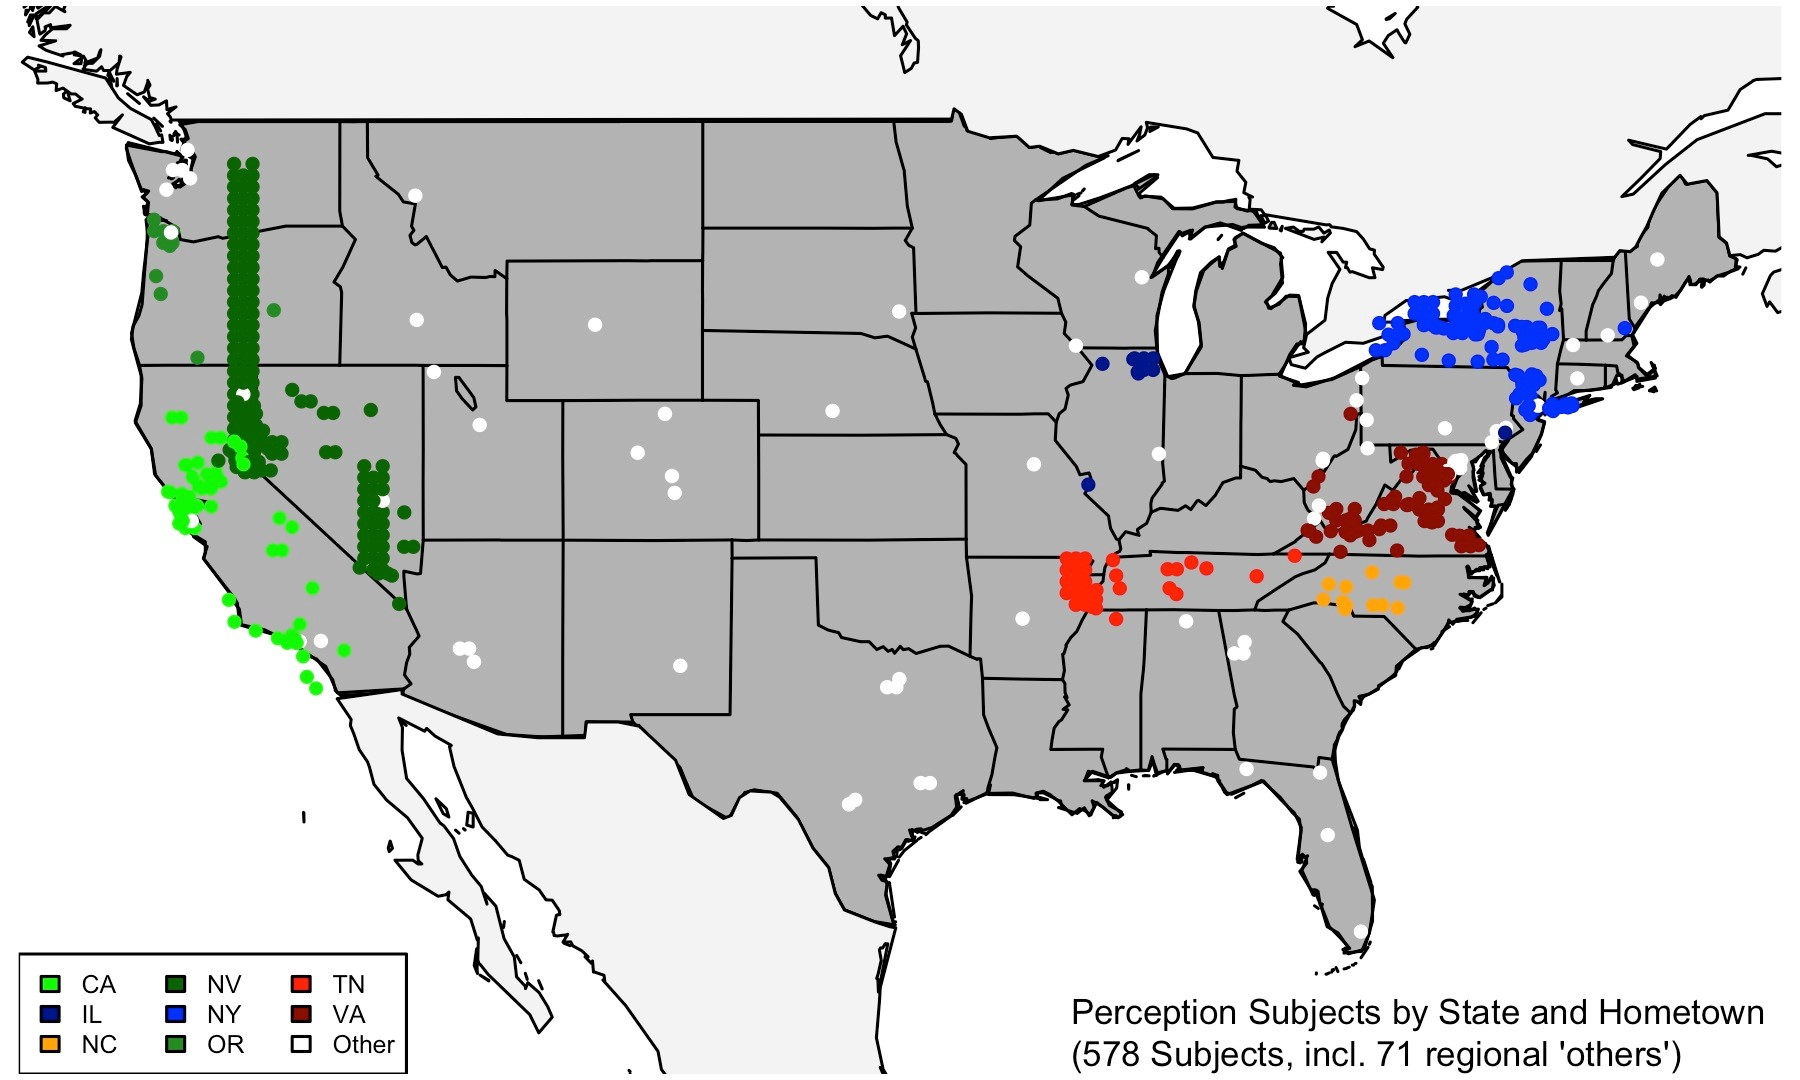
\includegraphics[width=\textwidth]{illustrations/kend_frid_fig1}
\caption{Location of 578 vowel identification participants. Colors indicate regional (i.e. U.S. state) associations for 507 participants included in our earlier work while white dots indicate participants not previously examined or assigned to a regional group; ``Stacks'' of dots indicate participants from same locale.}
\label{fig:kend:1}
\end{figure}

\subsection{Study design}
In the test, vowel tokens from a number of continua were randomly played for listeners who were then asked, in a forced-choice format, to indicate the token they just heard from two choices \citep{strange_cross-language_1995,thomas_sociophonetic_2002}. Each continuum range was synthesized into 7 steps based on a sample speaker’s production values for each of two selected endpoint vowel categories. The stimuli were created using estimated beginning and endpoint values for F1 and F2 for each vowel pair (based on regional vowel patterns). At each analysis frame, a distance in frequency was estimated between the trajectories of each vowel in the pair. Because duration was held constant, each vowel has the same number of analysis frames. Increments of change in frequency were estimated (using a linear interpolation) for consecutive steps of a 7-step continuum spanning the distance in F1 and F2 trajectories across the vowel pair. More information about the perception stimuli, as well as details exemplifying the synthesis (for the /e/{\textasciitilde}/ɛ/ test), is available in \citet{kendall_variation_2012}.


The sample speaker was a 40 year-old male from Reno, Nevada, who was chosen as representing unmarked dialectal features in line with \citet{clopper_acoustic_2004}. The tokens were embedded between a single consonant onset and single consonant coda (C\_C) and two consonant contexts were used for each vowel pair of interest (a post-bilabial context and a post-alveolar context, e.g. for /e/{\textasciitilde}/ɛ/, \textit{bait} \& \textit{bet} and\textit{ date} \& \textit{debt}). All following environments were alveolar obstruents. For the test, each trial presented a single vowel continuum step (played once) and participants were asked to indicate the token they just heard from two choices drawn from the relevant vowel categories (e.g. for the post-bilabial /e/{\textasciitilde}/ɛ/ test, \textit{bait} or \textit{bet}). To investigate how much of a role vowel dynamics plays in vowel category perception and whether this varies across dialects, two different conditions were created for each vowel continuum, one which altered dynamic information for each step along with steady state information and another which removed dynamic information. The static tokens were created with target formant values fixed based on midpoint values across the entire vowel trajectory while the dynamic tokens included the formant variability of the original tokens across time. Thus, the test included both versions for all vowels so that each participant’s vowel thresholds were measured in both static and dynamic contexts for the two different consonant contexts. 

\subsection{Test procedure}
In order to be simultaneously implemented across regions, the test was developed and administered through a website. Each step in each vowel continuum had four iterations – i.e. was played 4 times randomized over the course of the study. Thus, this vowel identification test included 20 perception continua over a total of 560 trials – 5 vowel pairs (/e/{\textasciitilde}/ɛ/, /i/{\textasciitilde}/ɪ/, /æ/{\textasciitilde}/ɑ/, /ʌ/{\textasciitilde}/o/, and /ɪ/{\textasciitilde}/u/) $\times$ 2 consonantal environments (post-bilabial and post-alveolar) $\times$ 2 conditions (static and dynamic) $\times$ 7 steps per continua $\times$ 4 repetitions. The study was also randomized by trial. 

\section{Analysis and results}

\subsection{Analysis}
In our previous work, we have focused entirely on subsets of our total perception data (primarily the tense and lax mid- and high-front vowels) and we have limited our examination to just European American participants from a set of specific sub-regions (and, as explained above, examined those participants in categorical regional groups). In this paper, we examine, for the first time, a more complete set of our perception data from the larger project: 20 perception continua for each of 578 participants from throughout the continental United States (participants in our database as of August 2014). 

As noted above, participants in the perception experiment heard vowels synthesized along a 7-step continuum and rated each step as one of two words in a minimal pair (e.g. \textit{bait} or \textit{bet}). The majority of our analyses have examined the data at this level through mixed-effect logistic regression (e.g. \citealt{kendall_variation_2012}). However, we can also examine the data in terms of the participants’ \isi{cross-over points} – the place in each 7-step continuum where a subject first “crossed over” the 50\% point of hearing predominately one vowel category to predominantly another. We chose this measure of the “first” point at which participants crossed over from recognition of one vowel quality to another to provide a more simple test case for the present analysis than assessing the full continuum data for stimuli set.\footnote{We also examined the cross-over data briefly in Kendall and Fridland (\citeyear{kendall_mapping_2010,kendall_variation_2012}).} Using a cross-over measure provides a single value for each stimuli set (henceforth also referred to as a variable) for each participant and is less complex as input for some of the methods we utilize in this paper. Future work can assess whether the geospatial techniques we employ can be usefully applied to, e.g., full logistic models of the continua data.

To exemplify the cross-over points and perception data more generally, \figref{fig:kend:2} illustrates the identification functions and cross-over points for /e/{\textasciitilde}/ɛ/ in the post-bilabial context (\textit{bait{\textasciitilde}bet}) for two individuals, Kim1111, a female from Memphis, TN in the South (on left), and Kristen147, a female from Rochester, NY in the Inland North (on right). Kim1111 highlights a Southern pattern for /e/{\textasciitilde}/ɛ/, with a relatively later cross-over in comparison to Kristen147, who shows a more Northern pattern, crossing-over to /ɛ/ earlier in the continuum \citep{kendall_variation_2012}.

\begin{figure}[t]
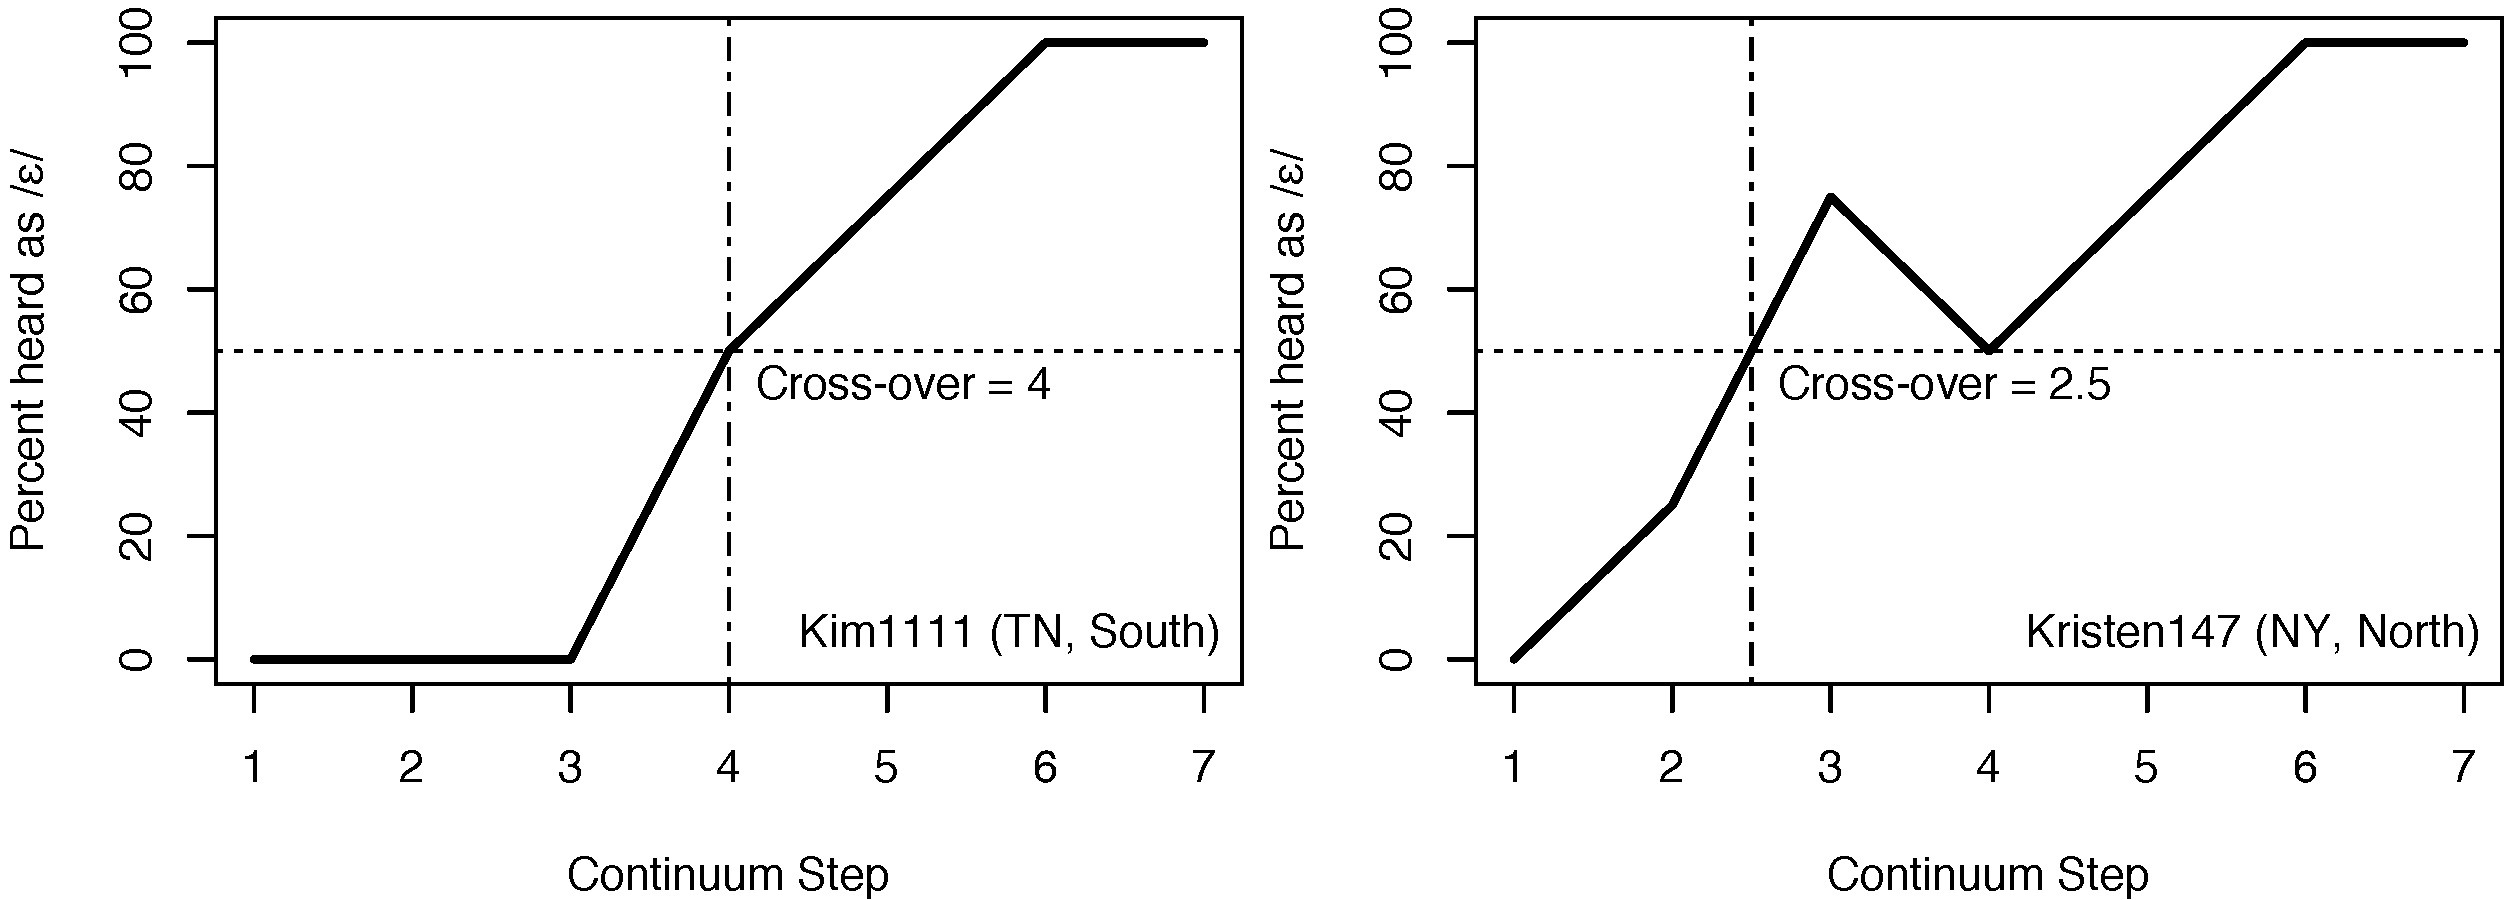
\includegraphics[width=\textwidth]{illustrations/kend_frid_fig2}
\caption{Identification function for /e/{\textasciitilde}/ɛ/ in dynamic post-bilabial context (\textit{bait}{\textasciitilde}\textit{bet}) for two individuals.}
\label{fig:kend:2}
\end{figure}
 
\largerpage
To begin to consider these cross-over data in more detail, we first examine the 507 speakers we have previously grouped into regional categories (South vs. North vs. West; these are the non-white dots in \figref{fig:kend:1}). \tabref{tab:kend:1} presents a breakdown of the results of a series of \isi{ANOVA} tests, which ask whether region differentiates cross-over points for each variable. The table shows results for Tukey post-hoc tests for the ANOVAs with \textit{p }values below 0.05. Due to the large number of statistical tests, it is judicious to use a Bonferroni corrected \textit{p }value as a more conservative measure of significance. Thus, while the table notes variables with \textit{p }values below 0.05 (noted by *), \textit{p }{\textless} 0.0025 (noted by **) is a better assessment of significance.

\tabref{tab:kend:1} also includes \isi{ANOVA} results for the first 3 Principal Components (PCs) from a Principal Components Analysis\is{principal components analysis} (PCA) for all 20 variables. PCA is a common dimensionality reduction and cluster analysis technique, and examining the Principal Components (PCs) provides a convenient way to assess trends across the whole (large) set of variables simultaneously. For sake of space, we do not discuss the PCA in depth here but note that PC1 accounts for 32.4\% of the variance, PC2 accounts for 14.8\%, and PC3 accounts for 11.0\%. Focusing on the individual variables (the first 5 rows of \tabref{tab:kend:1}), we see that ANOVAs yield \textit{p }{\textless} 0.05 for 11 of the 20 variables and \textit{p }{\textless} 0.0025 for 3 of these variables, the static and dynamic post-bilabial /e/{\textasciitilde}/ɛ/ continua and the dynamic post-alveolar /ʌ/{\textasciitilde}/o/ continuum. Overall, the majority of cases show the South having higher cross-over points than other regions, a finding inline with our results for the data examined elsewhere that showed, for example, Southerners tending to perceive /e/ farther along the synthesized F1/F2 continuum (e.g. \citealt{kendall_variation_2012}). The general finding of a difference between the South and the North in particular is confirmed in the results for the first two PCs. These patterns align with production differences in regional vowel patterns between the North and the South (e.g. \citealt{labov_atlas_2006-1}) and demonstrate that, similar to perception, perception is also sensitive to geographic identity \citep{fridland_exploring_2012}.

\begin{table}
\begin{tabular}{lllll}
\lsptoprule 
& {\bfseries Bilabial} &  & {\bfseries Alveolar} & \\
\cmidrule(lr){2-3}\cmidrule(lr){4-5}
{\bfseries Continuum} & {\bfseries Dynamic} & {\bfseries Static} & {\bfseries Dynamic} & {\bfseries Static}\\
\midrule
{\mdseries /i/ {\textasciitilde} /ɪ/} & {\mdseries {}-} & {\mdseries {}-} & {\mdseries * S {\textgreater} N, W} & {\mdseries * S {\textgreater} N}\\
{\mdseries /e/ {\textasciitilde} /ɛ/ } & {\mdseries ** S {\textgreater} N, W} & {\mdseries ** S {\textgreater} N, W} & {\mdseries * S {\textgreater} N, {\textasciitilde}W} & {\mdseries * S, W {\textgreater} {\textasciitilde}N}\\
{\mdseries /æ/ {\textasciitilde} /ɑ/ } & {\mdseries {}-} & {\mdseries {}-} & {\mdseries {}-} & {\mdseries * S {\textgreater} N, W}\\
{\mdseries  /ʌ/ {\textasciitilde} /o/} & {\mdseries {}-} & {\mdseries * S {\textgreater} {\textasciitilde}N} & {\mdseries ** S, W {\textgreater} N} & {\mdseries {}-}\\
{\mdseries /ɪ/ {\textasciitilde} /u/} & {\mdseries * S {\textgreater} W} & {\mdseries * S {\textgreater} W} & {\mdseries {}-} & {\mdseries {}-}\\
\midrule
{\mdseries PC1} & \multicolumn{4}{c}{ * S {\textless} N\par}\\
{\mdseries PC2} & \multicolumn{4}{c}{ * S {\textless} N, {\textasciitilde}W\par}\\
{\mdseries PC3} & \multicolumn{4}{c}{ {}-\par}\\
\lspbottomrule
\end{tabular}
\caption{Results for \isi{ANOVA} tests with Tukey post-hoc comparisons. - denotes region $p$ {\textgreater} 0.05; * denotes region $p$ {\textless} 0.05; ** denotes region $p$ {\textless} 0.0025; {\textgreater} indicates e.g. S {\textgreater} W = “South has a significantly higher cross-over than West”; {\textasciitilde} ~denotes marginally significant (0.075 {\textgreater} p {\textgreater} 0.05 post hoc comparison)}
\label{tab:kend:1}
\end{table}

Beyond noting differences in perception among the major regions of U.S. English, our present interest is in examining the perception data at a finer-level of regional granularity and to move away from our preexisting regional categories, which are based on production patterns and regional assignments from the \textit{ANAE} \citep{labov_atlas_2006-1}. We turn now to spatial autocorrelation techniques to ask whether we can learn anything new from examining the perception data from a geospatial perspective, where participants are considered in terms of the geospatial coordinates of their self-reported “hometowns” rather than as members of a predefined dialect region. 

Following Grieve (\citealt{grieve_corpus-based_2009}; \citealt{grieve_statistical_2011,grieve_multivariate_2013}) and previous work more generally on geospatial analysis (e.g. \citealt{moran_notes_1950,ord_local_1995}), we apply two geospatial analysis techniques to the cross-over point data. First, we use Moran’s \textit{I} statistic to ask whether (any of) the 20 variables show overall patterns of regional clustering. Moran’s \textit{I }provides a measure of global spatial autocorrelation, with associated \textit{p} values that indicate whether there are significant patterns of global (i.e. overall) spatial autocorrelation. Then, we apply Getis-Ord\is{Getis-Ord Gi} \textit{G}\textit{\textsubscript{i}}\textit{*} \textit{z }scores to measure local spatial autocorrelation to examine where any regional clusters appear to exist. These analyses are conducted using the spdep package for R \citep{bivand_spdep._2014}.

In this short paper, we limit our description of these methods and point readers to the sources mentioned above for a thorough explication of the techniques. As discussed in several papers by Grieve (see, for instance, \citealt{grieve_comparison_2014}), analysis for both Moran’s \textit{I} and Getis-Ord\is{Getis-Ord Gi} \textit{G}\textit{\textsubscript{i}}\textit{*} involve the choice of a \textsc{spatial weighting function}, which defines rules for how spatial relationships are assessed among the items being analyzed and which yields the \textsc{\isi{spatial distance matrix}} used for the analyses. There is no foolproof method for choosing the most appropriate \isi{spatial weighting function}. For the analyses here, we followed advice from \citet{bivand_creating_2014} and after assessing a range of different possible functions, used a binary spatial distance matrix using distances within 75\% of the maximum distance found from a k-nearest neighbors (kNN) analysis using k=7. Other measures, such as a full kNN (k=7) binary matrix, yielded similar, though not identical, results. Given the unevenness of the distribution of our participants over the U.S. (see again \figref{fig:kend:1}), the use of a binary kNN matrix seems most judicious. This somewhat limits skewing that might occur from other choices of matrix types, due to the fact that some groups of participants, like those from around Reno, NV where our sampling has been heaviest, have lots of close neighbors, while other participants, with hometowns farther afield from our sampling sites, have very few proximate neighbors. Further, since multiple participants self-reported the same hometowns (these were shown as stacks of dots in \figref{fig:kend:1}) and many geospatial analysis techniques require that each data point has a unique geospatial coordinate, the geospatial coordinates were jittered (using the R function jitter() with a factor of 0.05) to ensure that no coordinates where exactly identical.\is{geospatial autocorrelation|)}

For the Moran’s \textit{I }test, we find global spatial autocorrelation at \textit{p }{\textless} 0.0025 for six of the 20 perception variables. We do not find significant Moran’s \textit{I} results for any of the Principal Components\is{principal components analysis}, with PC1 obtaining a \textit{p} value of 0.095. The Moran’s \textit{I }results are shown in \tabref{tab:kend:2}. Thus, six of the variables are characterized as having global spatial clustering according to a conservative \textit{p} value assessment.

Getis-Ord\is{Getis-Ord Gi} \textit{G}\textit{\textsubscript{i}}\textit{*} analysis allows us to look at the spatial autocorrelation for each individual participant and to ask whether that participant is a member of a spatial cluster of like-valued participants. While examining all of the variables for local spatial autocorrelation would be useful, due to space constraints, we focus our attention on the dynamic variables which showed global spatial clustering by Moran’s \textit{I}. Maps for the static versions of these stimuli are not shown, despite that they also reached significance in the Moran’s \textit{I} analysis, also due to space limitations. Figures \ref{fig:kend:3}--\ref{fig:kend:6} display the Getis-Ord\is{Getis-Ord Gi} \textit{G}\textit{\textsubscript{i}}\textit{* }scores overlaid on maps of the U.S. for the three perception variables and for PC1. These maps depict the scores as colors (see the legend of each map for keys to the colors). Light gray lines on the maps indicate the neighbor relationships from the spatial weighting function, so clusters are assessed in terms of relationships between connected participants. These maps highlight important regional and sub-regional clusters. However, before discussing these clusters, we must also note that these clusters are best taken more as visual “suggestions” than as statistically significant proof of regional differences. The \textit{G}\textit{\textsubscript{i}}\textit{* }scores are effectively geospatially smoothed values for the variables (see e.g. \citealt[37]{grieve_multivariate_2013}). \citet{ord_local_1995} provide a measure of significance for \textit{G}\textit{\textsubscript{i}}\textit{* }values (here, for a dataset of this size, significant values should be {\textgreater} {\textasciitilde}{\textbar}3.72{\textbar}), but many of our mapped participants do not reach this level. Nonetheless, the maps can provide useful visual clues to fine-grained regional patterns and we see the \textit{G}\textit{\textsubscript{i}}\textit{*} scores as a tool for better understanding our data regardless of the degree of significance of the values obtained. \figref{fig:kend:3} displays the \textit{G}\textit{\textsubscript{i}}\textit{*} scores for /e/{\textasciitilde}/ɛ/ in the dynamic post-bilabial context, \figref{fig:kend:4} displays the scores for /ʌ/{\textasciitilde}/o/ in the dynamic post-alveolar context, and \figref{fig:kend:5} displays the scores for /ɪ/{\textasciitilde}/u/ in the dynamic post-bilabial context. Maps of static scores pattern similarly but, as stated above, are not included for sake of space. Again, while none of the PCs yielded significant Moran’s \textit{I} values, \figref{fig:kend:6} shows the \textit{G}\textit{\textsubscript{i}}\textit{*} scores for PC1, which helpfully capture some of the larger patterns across the maps.

\begin{table}[t]
\begin{tabular}{lllll}
\lsptoprule
& {\bfseries Bilabial} &  & {\bfseries Alveolar} & \\
\cmidrule(lr){2-3}\cmidrule(lr){4-5}
{\bfseries Continuum} & {\bfseries Dynamic} & {\bfseries Static} & {\bfseries Dynamic} & {\bfseries Static}\\
\midrule
{\mdseries /i/ {\textasciitilde} /ɪ/} & {\mdseries {}-} & {\mdseries {}-} & {\mdseries {\textasciitilde}} & {\mdseries {}-}\\
{\mdseries /e/ {\textasciitilde} /ɛ/ } & {\mdseries ** } & {\mdseries **} & {\mdseries {}-} & {\mdseries *}\\
{\mdseries /æ/ {\textasciitilde} /ɑ/ } & {\mdseries {}-} & {\mdseries {}-} & {\mdseries {\textasciitilde}} & {\mdseries *}\\
{\mdseries  /ʌ/ {\textasciitilde} /o/} & {\mdseries {}-} & {\mdseries {}-} & {\mdseries **} & {\mdseries **}\\
{\mdseries /ɪ/ {\textasciitilde} /u/} & {\mdseries ***} & {\mdseries ***} & {\mdseries {}-} & {\mdseries {}-}\\
\midrule
{\mdseries PC1} & \multicolumn{4}{c}{ {\textasciitilde}\par}\\
{\mdseries PC2} & \multicolumn{4}{c}{ {}-\par}\\
{\mdseries PC3} & \multicolumn{4}{c}{ {}-\par}\\
\lspbottomrule
\end{tabular}
\caption{Results for Moran’s I tests. {}- denotes not significant; {\textasciitilde} denotes 0.1 {\textgreater} $p$ {\textgreater} 0.05; * denotes $p$ {\textless} 0.05; ** denotes $p$ {\textless} 0.0025 (Bonferroni corrected significant p value); *** denotes $p$ {\textless} 0.00001}
\label{tab:kend:2}
\end{table}

 
\begin{figure}
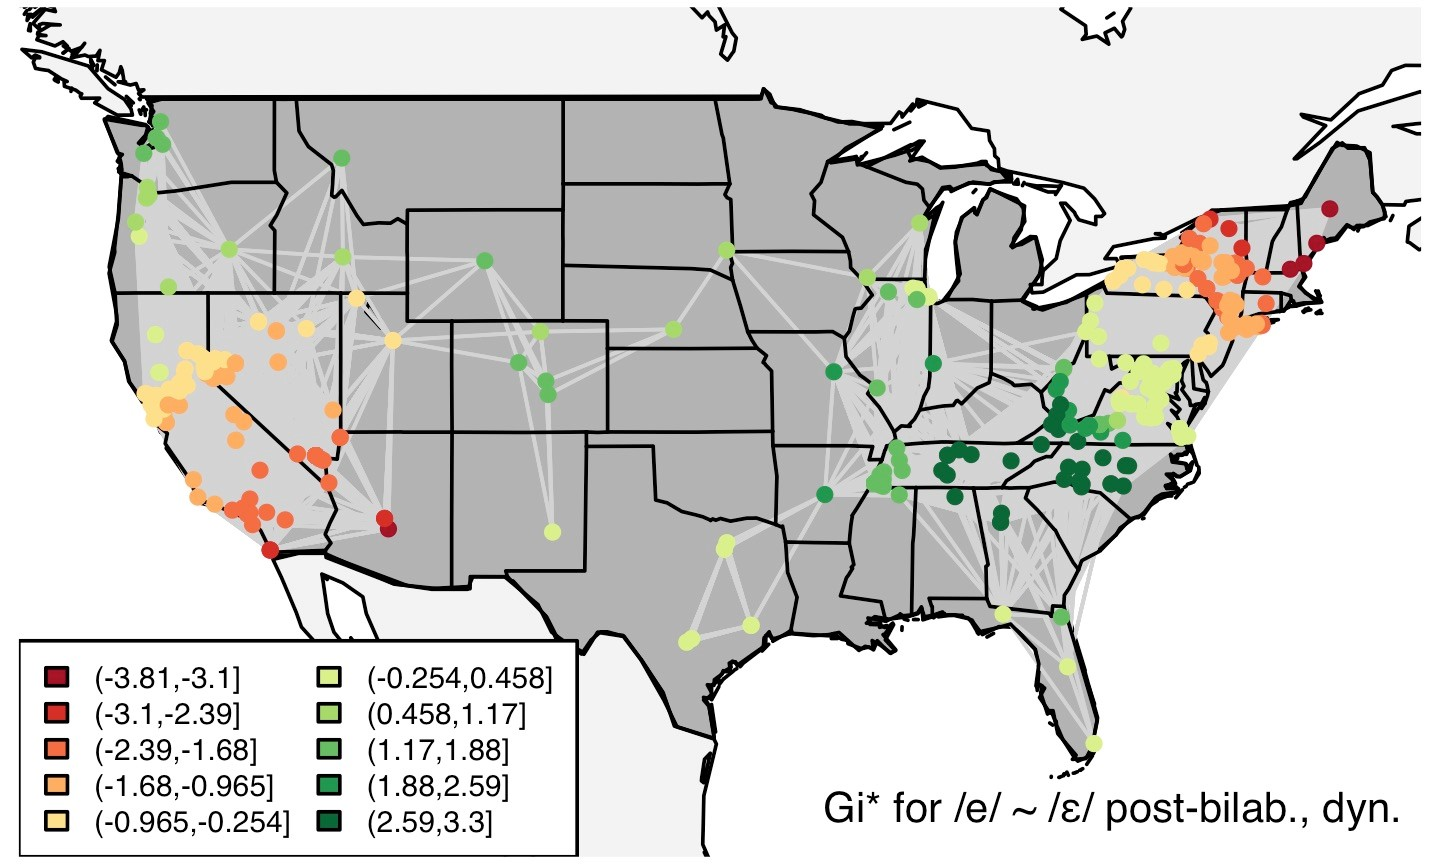
\includegraphics[width=\textwidth]{illustrations/kend_frid_fig3}
\caption{Getis-Ord G\textsubscript{i}* $z$ score values for /e/{\textasciitilde}/ɛ/ in the dynamic post-bilabial context.}
\label{fig:kend:3}\is{Getis-Ord Gi}
\end{figure}

\begin{figure}
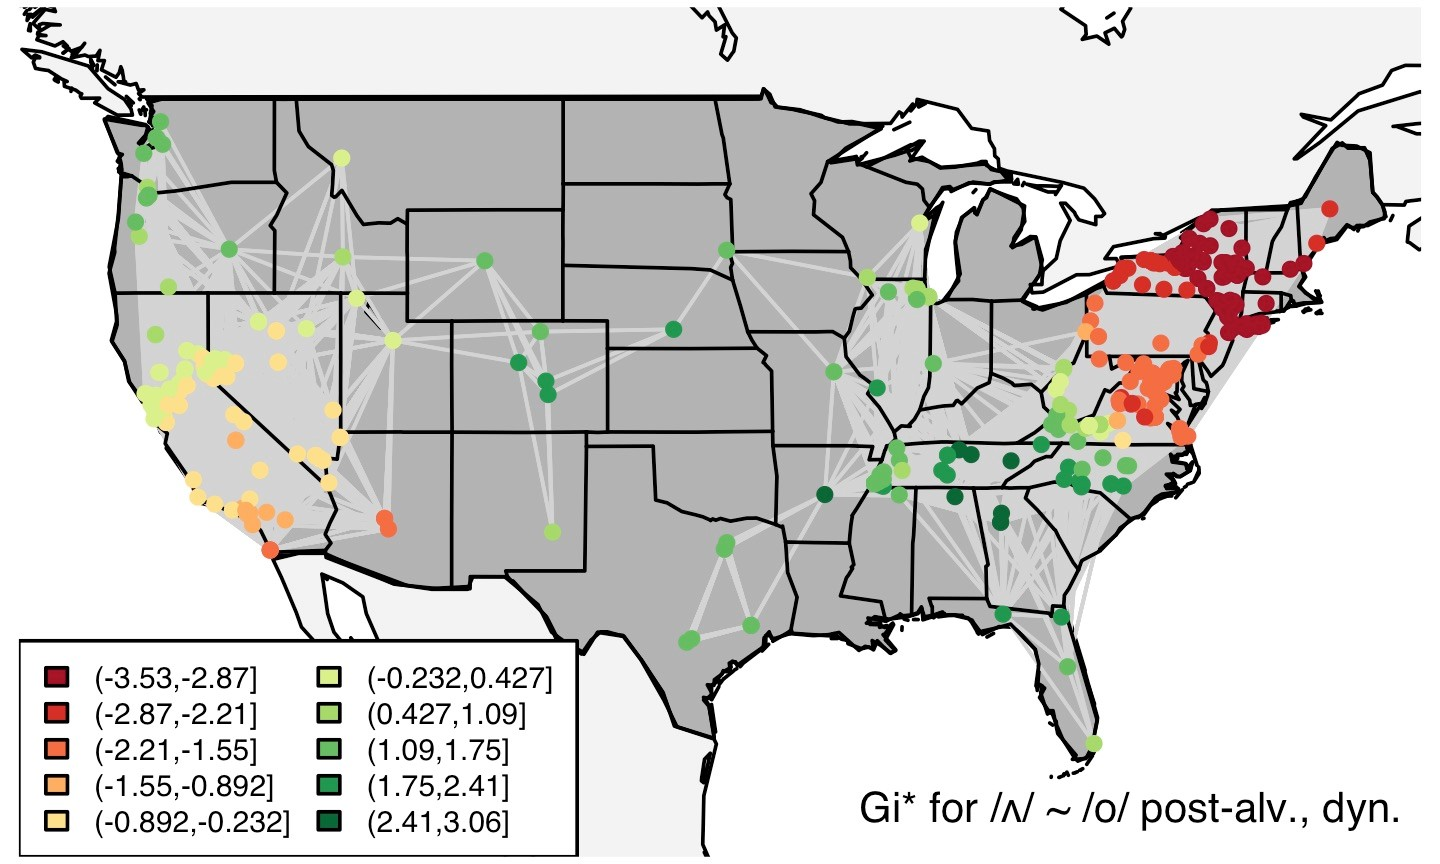
\includegraphics[width=\textwidth]{illustrations/kend_frid_fig4}
\caption{Getis-Ord G\textsubscript{i}* $z$ score values for /ʌ/{\textasciitilde}/o/ in the dynamic post-alveolar context.}
\label{fig:kend:4}\is{Getis-Ord Gi}
\end{figure}

\begin{figure}
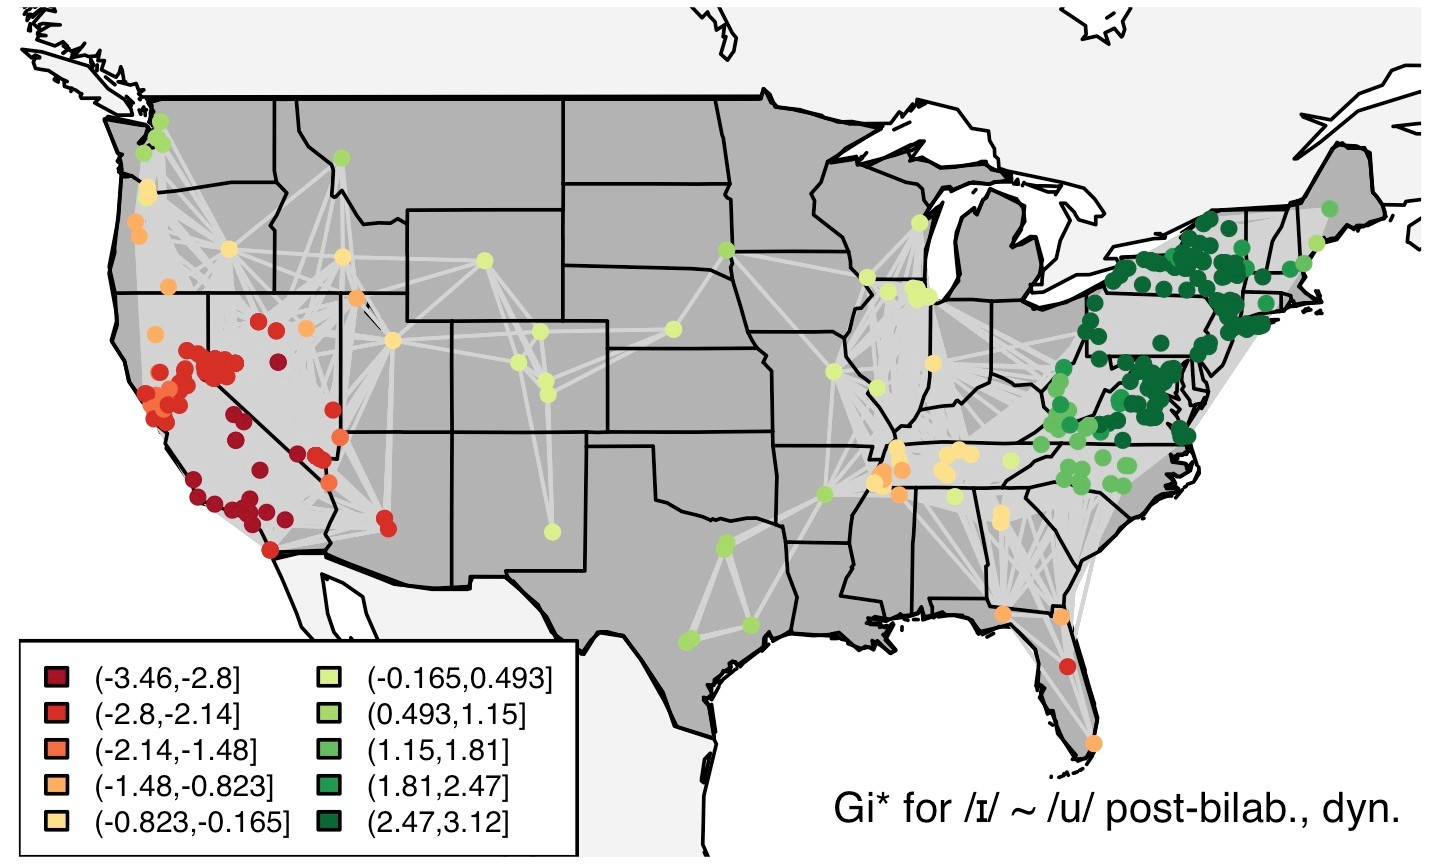
\includegraphics[width=\textwidth]{illustrations/kend_frid_fig5}
\caption{Getis-Ord G\textsubscript{i}* $z$ score values for /ɪ/{\textasciitilde}/u/ in the dynamic post-bilabial context.}
\label{fig:kend:5}\is{Getis-Ord Gi}
\end{figure}

\begin{figure}
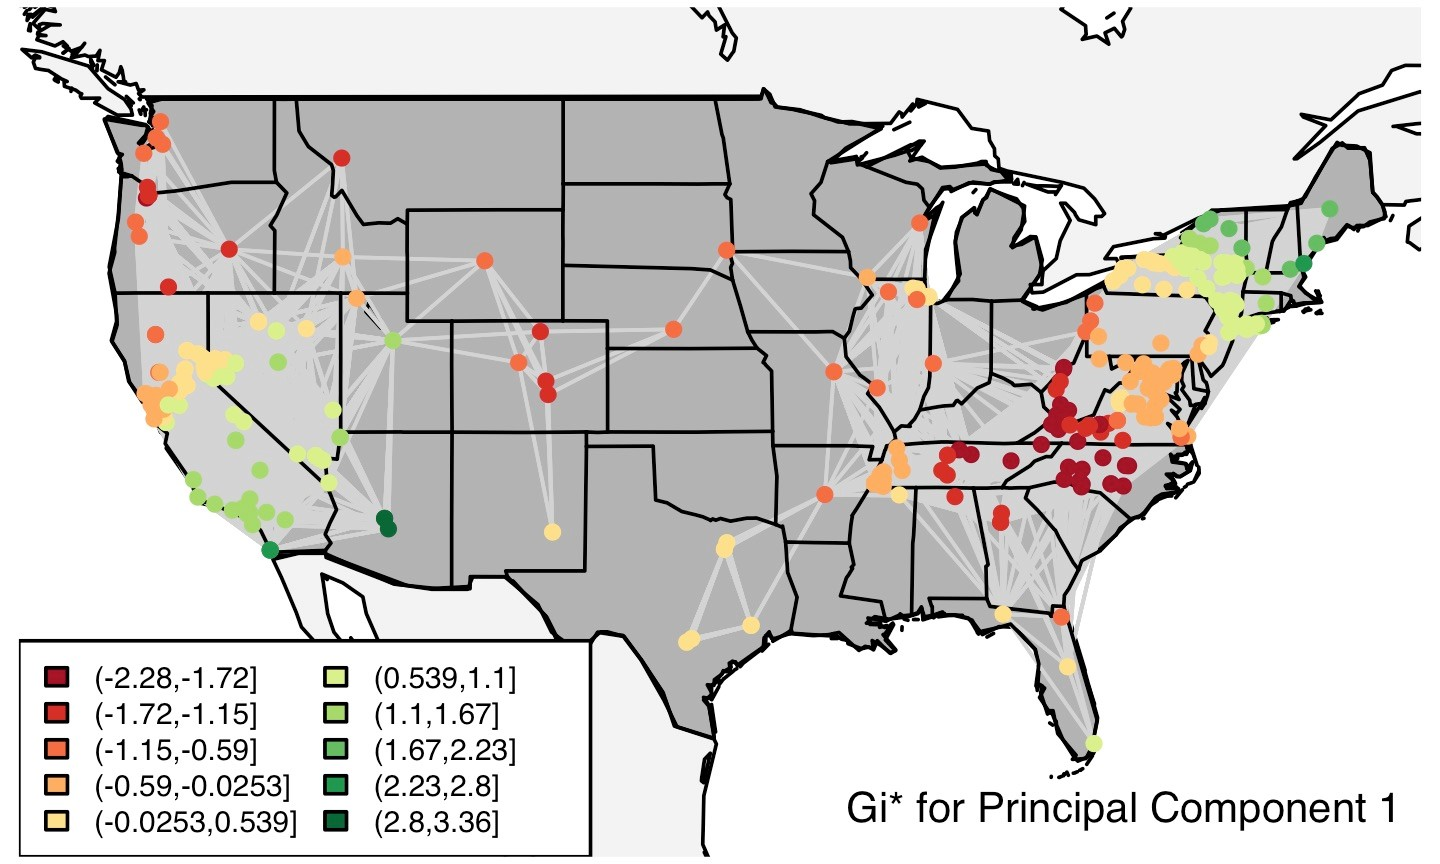
\includegraphics[width=\textwidth]{illustrations/kend_frid_fig6}
\caption{Getis-Ord G\textsubscript{i}* $z$ score values for Principal Component 1.}
\label{fig:kend:6}\is{Getis-Ord Gi}
\end{figure}

\subsection{Discussion}
To a large degree, the Getis-Ord\is{Getis-Ord Gi} maps demonstrate that speakers within traditionally defined dialect regions often pattern perceptually similarly to each other. Altogether, however, the maps also suggest some finer-grained patterns of interest. We see in these maps that perceptual similarity is not simply aligned with traditional regional divisions – there are a number of intra-regional and cross-regional perceptual clusters. It must be remembered, however, that the mapped patterns are based on heterogeneous samples across the U.S. (with large clusters of participants in areas around Reno, NV, Oswego, NY, and Memphis, TN). Though strong generalizations cannot be made from our data at this point, we can, however, point to some suggestive findings.

First, throughout the maps we see a visual break between our participants in Southern California and those from the rest of the West Coast. We also notice that in all the maps, California and Nevada speakers appear to cluster together more than they cluster with other areas in the West. Figures 3, 4, and 5 all show less clustering with the Pacific Northwest region in particular (as well as several Inland Western states such as Colorado, Wyoming, and Idaho). Similarly, while our cross-over analysis reported earlier in this paper displayed significant differences overall mainly with the way our Southerners perceptually behave compared to other regions, we see in Figures 3, 4, and 6, that sub-regional clusters in the Eastern U.S. and among our Southern site participants suggest that more subtle intra-regional differences in perceptual behavior may also be important to explore.  

Looking at these maps without preconceived regional boundaries would lead one to a somewhat different view of shared perceptual behavior than one takes away from imposing traditional dialectological constructs based on production (as we have done in our previous work). For example, although often lumped together according to production norms such as the low back vowel merger into one “Western dialect” region (e.g. in \textit{ANAE}), our Western participants show substantial differences in perceptual clustering. Such clustering is suggestive that dialect, as conceived perceptually, may indeed need to be explored as something different than that of dialect expressed in production, as suggested by Sumner and Samuel’s (\citeyear{sumner_effect_2009}) work. In other words, while “regional” clustering in perception is clear in these maps, perceptual patterns generally fall into smaller clusters than the macro-level regional groups we might assume based on broader generalizations, as we discuss a bit more below. Certainly, while production differences within, in addition to across, regions have been noted in dialectological work, pan-regional vowel shifts, characterizing wide swaths of regions, have been widely researched in recent years.  

What emerges overall from these maps is an indication that perceptual similarity and difference may not so cleanly align with traditional dialect regions (based on production), despite the fact that we often impose region as a super-ordinate categorizing tool. As mentioned above, the Getis-Ord\is{Getis-Ord Gi} maps generally show that speakers in our sites in the West and the South are not perceptually unified in a way that we might expect given claims about production tendencies (e.g. such as the California Vowel Shift\is{California vowel shift} or the Southern Vowel Shift\is{Southern vowel shift}) in those regions \citep{labov_atlas_2006-1}. While these differences are necessarily putative at this point, they do suggest that perception needs to play a role in our understanding of dialect.   

Though beyond the scope of this paper to consider in detail, it may be that many of these perceptual differences, like production differences, correlate with historical migratory and settlement patterns. For example, the history of Southern Californian speech influences does stand in contrast with that of Northern California, owing to greater Southern and Spanish influence. In addition, geographic boundaries effectively limited early North-South travel along the West Coast, leading to sharp differences in lexical patterns in traditional dialect maps for the area \citep{bright_word_1967,reed_problems_1972}. Nonetheless, what is intriguing in the mapping of our perception study results using geospatial techniques is that we can see such influences affecting how sounds are heard, not just produced. 

Likewise, perceptual clusters of speakers are also notable within the South – in parts of Middle and Eastern Tennessee and in inland North Carolina and Virginia – which suggest these participants hear the perceptual continuum more similarly than other residents of their own states. For example, our subjects from Memphis (Western Tennessee) show different perceptual tendencies than subjects from Eastern Tennessee. This could partly reflect early settlement patterns and, importantly, contemporary migratory differences within the state. It is perhaps not surprising that such differences emerge, but it reinforces our sense that people use dialect variation to establish place rather than place establishing dialect.

However, we end here and do not attempt to elucidate the reasons for these differences more deeply as to do so would be too speculative at this stage. What is clear is that perception, like production, is a place-based phenomenon, with place here reflecting geo-social similarity and not just superimposed regional categorization. While our preliminary analysis has been suggestive of areas within our data we plan to explore more deeply, our goal here has been a more general one – to assess the benefit of looking at perceptual data using geospatial analysis.\is{geospatial autocorrelation}

\section{Conclusion}
Overall, this investigation has shown that \is{dialectometry|(}dialectometry has a lot to offer the investigation of regional patterns in perception. We gain new insights in the perception of linguistic form by assessing the geospatial patterns of the responses made by participants in perception experiments. The clusters appear to not simply align with regionally demarking isoglosses coming from more traditional dialect surveys, or even the recent phonological survey of \textit{The \isi{Atlas of North American English}} \citep{labov_atlas_2006-1}.

\largerpage[-1]
While the visual patterns in the maps of Figures 3-6 are suggestive of finer regional patterns in perception than we have previously considered, it must be remembered that these patterns are only suggestive. Further analysis and more regionally diverse and balanced data are needed to assess the extent to which these clusters are meaningfully different from one another. We hope that this further analysis will involve increased use of techniques from dialectometry\is{dialectometry|)} so that we can better assess the extent to which isoglosses in perception align with those in production.\footnote{Although we leave most of this further analysis for the future, we have begun to follow up on the pattern observed from the Getis-Ord\is{Getis-Ord Gi} analysis that Southern California differs from the rest of the West Coast. A linear regression on just participants from the West Coast (participants from longitudes west of -116.54º, the longitude of our east-most Californian participant) indeed identifies a significant relationship between latitude coordinate and e.g. perception of the /e/{\textasciitilde}/ɛ/ dynamic post-bilabial continuum (coef=0.1278, \textit{p} {\textless} 0.05) and conditional inference trees find significant breaks at about latitude 39º for many of the continua. We also find significant differences for sub-groupings of West Coast participants based on several separations of these participants into “North” and “South” West Coast based on the visual differences in Figures 3-6.}

\section*{Acknowledgements}
This research has been supported by grants \# BCS-0518264 \& BCS-1123460 (PI Fridland), and BCS-1122950 (PI Kendall) from the National Science Foundation. We thank Craig Fickle and Charlie Farrington at the University of Oregon, and Sohei Okamoto and Kaylynn Gunter at the University of Nevada, Reno, for support with various aspects of this research. We also thank our audience at Methods in Dialectology XV, the editors, and the three anonymous reviewers for their helpful advice about our project.

\printbibliography[heading=subbibliography,notkeyword=this]
\end{document}